\colorlet{species background color}{black!15}
\tikzset{
    x={1pt},
    y={-1pt},
    species border/.style={
        line width={1pt},
        shorten <={-1pt / 2 + 0.05pt},
        shorten >={-1pt / 2 + 0.05pt},
    },
    species background/.style={
        fill=species background color,
        draw=species background color,
        line width={1pt},
        rounded corners,
    },
    species label/.style={
        font=\bfseries,
        midway,
        anchor=west,
        xshift=10
    },
    branch/.style={
        draw={#1},
        line width={0.5pt},
    },
    transfer branch/.style={
        branch={#1},
        -Stealth,
    },
    loss/.style={
        draw={#1}, cross out, thick,
        line width={0.5pt},
        inner sep=0pt,
        outer sep=0pt,
        minimum width={3},
        minimum height={3},
    },
    extant gene/.style 2 args={
        circle, fill={#1},
        outer sep=0pt, inner sep=0pt,
        minimum size={3},
        label={
            [font={\color{#1}},
                align=center,
                inner xsep=4pt, inner ysep=0pt,
                outer xsep=0pt, outer ysep=0pt]
            right:#2
        },
    },
    extant gene/.default={black}{},
    branch node/.style={
        draw={#1}, fill={species background color!50!white},
        align=center,
        font={\color{#1}},
        outer sep=0pt, inner xsep=0pt, inner ysep=2pt,
        line width={0.5pt},
    },
    branch node/.default={black},
    speciation/.style={
        branch node={#1}, rectangle, rounded corners,
        inner xsep=4pt,
        minimum width={8},
        minimum height={8},
    },
    duplication/.style={
        branch node={#1}, rectangle,
        inner xsep=4pt,
        minimum width={8},
        minimum height={8},
    },
    horizontal gene transfer/.style={
        branch node={#1}, chamfered rectangle,
        chamfered rectangle sep={8 / 2.4},
        inner xsep=2pt,
        inner ysep=-1pt,
        minimum width={8},
        minimum height={8},
    },
}
\definecolor{reccolor0}{HTML}{000000}
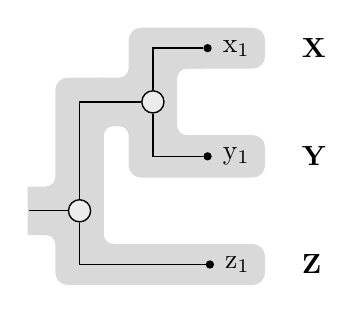
\begin{tikzpicture}
% background
\path[species background] (26.5,18.05997) -- (10,18.05997) -- (10,57.41996) [sharp corners] -- (0,57.41996) -- (0,73.91996) [rounded corners] -- (10,73.91996) -- (10,91.97993) [sharp corners] -- (53.84,91.97993) [rounded corners] -- (63.84,78.16996) -- (26.5,78.16996) -- (26.5,34.55997) [sharp corners] -- (36.5,34.55997) -- cycle;
\path[species background] (53.0,0) -- (36.5,0) -- (36.5,18.05997) [sharp corners] -- (26.5,18.05997) -- (26.5,34.55997) [rounded corners] -- (36.5,34.55997) -- (36.5,53.16996) [sharp corners] -- (53.0,53.16996) [rounded corners] -- (63.0,38.80997) -- (53.0,38.80997) -- (53.0,13.80997) [sharp corners] -- (63.0,13.80997) -- cycle;
\path[species background] (53.0,0) -- (84.763,0) -- (84.763,13.80997) -- (53.0,13.80997);
\path[species background] (53.0,38.80997) -- (84.763,38.80997) -- (84.763,53.16996) -- (53.0,53.16996);
\path[species background] (53.84,78.16996) -- (84.763,78.16996) -- (84.763,91.97993) -- (53.84,91.97993);
% species
\path[species border] (26.5,18.05997) -- (10,18.05997) -- (10,57.41996) -- (0,57.41996);
\path[species border] (53.84,91.97993) -- (10,91.97993) -- (10,73.91996) -- (0,73.91996);
\path[species border] (26.5,34.55997) -- (26.5,34.55997) -- (26.5,78.16996) -- (53.84,78.16996);
\path[species border] (53.0,0) -- (36.5,0) -- (36.5,18.05997) -- (26.5,18.05997);
\path[species border] (53.0,53.16996) -- (36.5,53.16996) -- (36.5,34.55997) -- (26.5,34.55997);
\path[species border] (53.0,13.80997) -- (53.0,13.80997) -- (53.0,38.80997) -- (53.0,38.80997);
\path[species border] (53.0,0) -- (84.763,0) -- node[species label] {X} (84.763,13.80997) -- (53.0,13.80997);
\path[species border] (53.0,38.80997) -- (84.763,38.80997) -- node[species label] {Y} (84.763,53.16996) -- (53.0,53.16996);
\path[species border] (53.84,78.16996) -- (84.763,78.16996) -- node[species label] {Z} (84.763,91.97993) -- (53.84,91.97993);
% gene branches
\path[branch={reccolor0}] (14,65.66996) -- (0,65.66996);
\draw[branch={reccolor0}] (26.5,26.30997) -| (18.25,61.41996) (18.25,69.91996) |- (53.84,85.074945);
\path[branch={reccolor0}] (40.5,26.30997) -- (26.5,26.30997);
\draw[branch={reccolor0}] (53.0,6.904985) -| (44.75,22.05997) (44.75,30.55997) |- (53.0,45.989965000000005);
\path[branch={reccolor0}] (63.0,6.904985) -- (53.0,6.904985);
\path[branch={reccolor0}] (63.0,45.989965000000005) -- (53.0,45.989965000000005);
\path[branch={reccolor0}] (63.84,85.074945) -- (53.84,85.074945);
% gene transfers
% events
\node[speciation={reccolor0}] at (18.25,65.66996) {};
\node[speciation={reccolor0}] at (44.75,26.30997) {};
\node[extant gene={reccolor0}{x\textsubscript{1}}] at (64.5,6.904985) {};
\node[extant gene={reccolor0}{y\textsubscript{1}}] at (64.5,45.989965000000005) {};
\node[extant gene={reccolor0}{z\textsubscript{1}}] at (65.34,85.074945) {};
\end{tikzpicture}
